\subsection{Cost: the price of the certificate, and how cross-fitting lowers it}\label{sec:res-cost}

\textbf{Split design.} The decision-aware split alarm (CNA-DA, $\alpha_{\max}=0.10$) kept its failure rate at or below $\alpha_{\max}$ in every lead-time and cost-ratio cell with a positive lead time (largest 6.1\,\%; H4b supported) and failed on 1.8\,\% of units over all cells and repetitions. It was cheaper than age replacement on PHM08, FD002, FD004 and the battery cells (12--16 of 16 cells; never significantly dearer anywhere), than the probability-threshold policy with threshold $1/\rho$ on PHM08, FD002 and FD004, and than the optimised probability-threshold policy on PHM08, FD001 and the battery cells (8 of 16 cells each). It was not the cheapest policy (H4 not supported): a cost-tuned alarm with a one-standard-error rule was cheaper in 8 of 16 cells on FD001 and 11 on FD003, and the capacity trend was the cheapest policy on the battery cells. Proposition~\ref{prop:cost}(ii) explains most of the gap: with 32 calibration units no order-statistic level fails less often than 3\,\%, and at $\rho=50$ each such failure costs as much as 49 planned replacements; the cost ratios against the one-standard-error rule grew with $\rho$ and were largest on the two datasets with 32 calibration units (FD001 and FD003; median ratio 1.37 and 1.45) and smallest on those with 70--83 (PHM08 and FD002; 1.00 and 1.04).

\textbf{Cross-fitting.} Calibrating on all training units by cross-fitting attacks that floor directly. The cross-fitted alarm CNA+ at $\alpha=0.10$ failed on 3.8--10.1\,\% of test units at the primary lead time (repetition~0; H7a supported; 4.3--10.1\,\% averaged over the three repetitions), within the nominal level on every dataset although Theorem~\ref{thm:cvplus} guarantees only $2\alpha$ plus a finite-$K$ term, and it gave the same notice as the split alarm (median 15--22 engine cycles; battery 42). Its decision-aware version was cheaper than the split CNA-DA on FD001, FD003 and FD004 (8--12 of 16 cells, never dearer) and mixed elsewhere, so the protocol's prediction of at least four datasets (H7b) was not met. Its mean excess cost over the cheapest policy in each cell fell to 0.4--19.5\,\% (from 8.5--85.6\,\% for the split version; Table~\ref{tab:cost}, Fig.~\ref{fig:cvplus}b).

\textbf{Equal information.} The comparison above favours CNA+, which calibrates on all training units while the uncertified policies were tuned on the 60/40 split. The third protocol therefore rebuilt the comparators on exactly the same five fold models: selected on the out-of-fold predictions of all training units and applied through the average of the five models (CF in Table~\ref{tab:cost}). With equal information the certified alarm cost about as much as the best uncertified rules (H9). Its mean excess over the cheapest of the six policies in this comparison was 1.0--14.3\,\% across the seven datasets, against 0.6--11.0\,\% for the one-standard-error cost-tuned alarm and 1.8--13.5\,\% for policy~1 of Kamariotis et al.\ with an optimised threshold. Averaged over the three repetitions (descriptive) the three ranges were 1.9--14.6, 0.9--11.7 and 1.9--11.8\,\%, and the excess of CNA+-DA moved by up to 12 points between repetitions (N-CMAPSS), so differences of a few points among these three policies are within the variability of the split. By the protocol's cell-count rule CNA+-DA was never dearer than either: it was cheaper than the one-standard-error alarm on the battery cells (16 of 16 cells) and on FD004 (8 of 16) and mixed on the other five datasets, and mixed against the optimised probability-threshold policy on all seven. It was cheaper than policy~1 with the heuristic threshold $1/\rho$ on PHM08, FD002 and FD004. Plain cost tuning won many cells by small margins but lost heavily in a few, because it occasionally chose a setting at the edge of the feasible region: its largest excess in a cell was 97\,\% on FD003, against 45\,\% for CNA+-DA. Where CNA+-DA did lose, it lost at $\rho=50$: with about 80 calibration units its failure probability cannot fall below about 1.2\,\% (Proposition~\ref{prop:cost}), and the one-standard-error alarm, which can choose levels beyond the most demanding calibration unit, had no test failure in those cells. The one-standard-error and optimised-threshold comparators failed on 0--1\,\% of test units at the primary lead time and $\rho=10$ (all three repetitions), the heuristic threshold on 3.3--13.1\,\%; the former achieved low failure rates on these units, but without a guarantee for the next one.


\begin{table*}[t]\footnotesize\setlength{\tabcolsep}{4pt}
\caption{Mean excess cost over the cheapest policy in each of the 16 lead-time and cost-ratio cells (\%; cross-validation, repetition~0). Rows~1--3 are certified; the others are not. ``CF'': selected on cross-fitted out-of-fold predictions of all training units and applied through the average of the same five fold models as CNA+ (equal information with CNA+); the split policies use 60\,\% of the training units for fitting and 40\,\% for selection.}\label{tab:cost}
\resizebox{\textwidth}{!}{%
\begin{tabular}{@{}llllllll@{}}
\toprule
Policy & PHM08 & FD001 & FD002 & FD003 & FD004 & N-CMAPSS & Battery \\
\midrule
CNA-DA, split (certified) & 8.5 & 64.3 & 13.6 & 85.6 & 19.9 & 50.4 & 30.4 \\
CNA+-DA, cross-fitted (certified, $2\alpha$ bound) & 6.9 & 9.0 & 0.4 & 13.1 & 1.9 & 5.6 & 19.5 \\
CNA-DA on capacity trend (certified) & -- & -- & -- & -- & -- & -- & 18.8 \\
Cost-tuned STW, 1-SE, split & 0.9 & 0.7 & 4.6 & 6.2 & 2.8 & 51.2 & 6.1 \\
Window-tuned STW, split & 2.0 & 36.3 & 4.1 & 38.6 & 13.9 & 29.3 & 29.8 \\
Policy 1, optimised, split & 4.4 & 51.9 & 8.3 & 42.7 & 16.8 & 12.9 & 27.1 \\
Capacity trend, 1-SE & -- & -- & -- & -- & -- & -- & 1.9 \\
Age replacement & 80.6 & 72.9 & 57.6 & 89.5 & 80.8 & 18.8 & 179.7 \\
\midrule
\multicolumn{8}{@{}l}{\emph{Equal information with CNA+ (same five fold models; excess over the cheapest of these six policies; policy 1 with threshold $1/\rho$ not shown)}} \\
CNA+-DA (certified) & 8.9 & 14.3 & 1.0 & 12.8 & 3.8 & 13.0 & 1.5 \\
Cost-tuned STW, 1-SE, CF & 0.6 & 1.0 & 1.1 & 0.8 & 1.2 & 11.0 & 7.6 \\
Cost-tuned STW, plain, CF & 6.0 & 18.6 & 6.7 & 21.7 & 6.7 & 19.6 & 1.3 \\
Policy 1, optimised, CF & 4.3 & 9.9 & 1.8 & 13.5 & 3.4 & 10.4 & 2.0 \\
Age replacement & 84.2 & 81.0 & 58.5 & 89.2 & 84.6 & 26.8 & 132.5 \\
\bottomrule
\end{tabular}}

\end{table*}

\subsection{The setting and metric of Kamariotis et al.}\label{sec:res-m}

On their decision grid (decisions every 10 cycles, no lead time) and with their metric $M$, the split CNA-DA reached $M$ = 11.9--34.1\,\% at $c_p/c_c=0.1$ on PHM08 and FD001--FD004 (Table~\ref{tab:m}, Fig.~\ref{fig:cvplus}c). It was better than their policy~1 with an optimised threshold on FD001 ($-1.3$ points, paired 95\,\% interval $-2.0$ to $-0.7$) and indistinguishable from it on the other four datasets, better than policy~1 with the heuristic threshold $c_p/c_c$ on FD004, and better than age replacement on all five. The cost-tuned alarm with the one-standard-error rule had the lowest $M$ on every dataset (4.4--18.1\,\%) and was significantly better than CNA-DA on FD002 and FD004. At $c_p/c_c=0.02$ the floor of Proposition~\ref{prop:cost} dominates: with 32--83 calibration units, a certified failure probability of 1--3\,\% costs as much as 50 preventive replacements per failure, and CNA-DA's $M$ rose to 50--159\,\%, close to that of policy~1 (27--156\,\%), against 4--61\,\% for the one-standard-error rule. The comparison is in our implementation of their policy, with their probability model replaced by an empirical one built from our regressor, and on our splits; the values they report come from other models on a single 20-engine split and are not comparable.

\begin{table}[t]\footnotesize\setlength{\tabcolsep}{3pt}
\caption{Metric $M$ (\%) in the setting of Kamariotis et al.\ ($\Delta T=10$ cycles, no lead time, $c_p/c_c=0.1$; five-fold cross-validation, repetition~0) and, in brackets, test failures.}\label{tab:m}
\resizebox{\linewidth}{!}{%
\begin{tabular}{@{}llllll@{}}
\toprule
Policy & PHM08 & FD001 & FD002 & FD003 & FD004 \\
\midrule
CNA-DA (certified, $\alpha_{\max}=0.10$) & 11.9 (2) & 30.2 (3) & 20.6 (5) & 33.0 (3) & 34.1 (7) \\
CNA, $\alpha=0.05$ (certified) & 43.6 (10) & 30.2 (3) & 39.6 (11) & 33.0 (3) & 80.5 (21) \\
Policy 1, optimised threshold & 8.3 (1) & 31.4 (3) & 17.7 (4) & 25.4 (2) & 30.9 (6) \\
Policy 1, threshold $c_p/c_c$ & 18.9 (4) & 48.8 (5) & 23.4 (6) & 39.0 (4) & 77.2 (20) \\
Cost-tuned STW, 1-SE & 4.4 (0) & 6.1 (0) & 5.3 (0) & 18.1 (1) & 17.8 (2) \\
Age replacement & 64.2 (1) & 79.3 (1) & 73.5 (2) & 73.0 (0) & 91.7 (1) \\
\bottomrule
\end{tabular}
}
\end{table}

\begin{figure*}[t]\centering
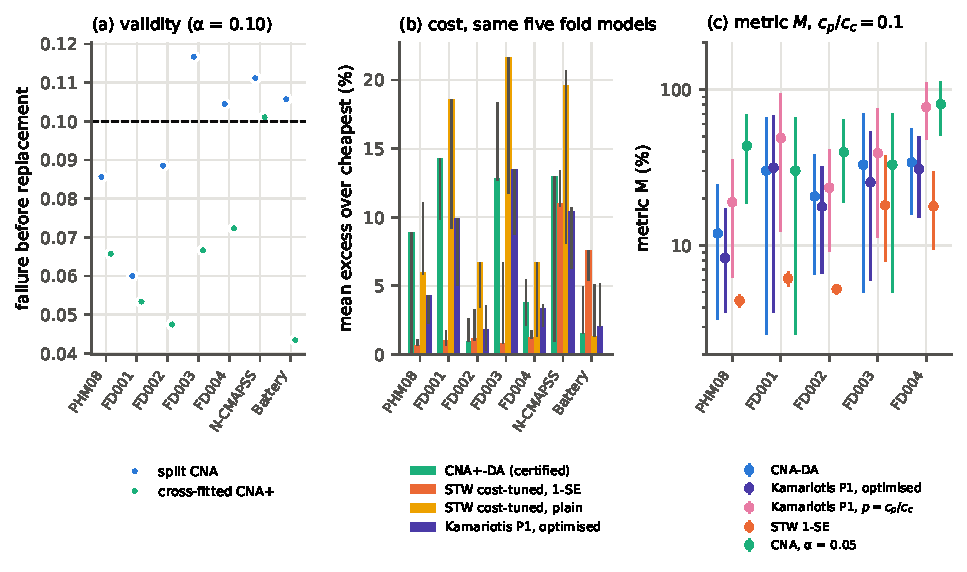
\includegraphics[width=0.95\textwidth]{figures/Fig7_cvplus_M.pdf}
\caption{(a) Failure before replacement at $\alpha=0.10$ and the primary lead time for the split (CNA) and cross-fitted (CNA+) alarms. (b) Mean excess cost over the cheapest policy in each of the 16 cells for the cross-fitted certified alarm and the uncertified policies built on the same five fold models (equal information); bars: repetition~0, lines: range over the three repetitions. (c) Metric $M$ in the setting of Kamariotis et al.\ at $c_p/c_c=0.1$ with paired-bootstrap 95\,\% intervals (log scale).}\label{fig:cvplus}
\end{figure*}
